\graphicspath{{./gui/Bilder/}}

\chapter{Arbeitspaket GUI}
Für die Analyse, den Entwurf, die Implementierung dieses Arbeitspaketes übernahm Herr Krause die Verantwortung. Während der Integration des Arbeitspaketes waren die Herren Krupinski und Schleinkhofer unterstützend eingebunden.
\paragraph{}
In der Projektspezifikation wurde die Anforderung der Visualisierung der Motor-Charakteristiken und der Steuerung des Motors mit aufgenommen. Zu diesem Zweck wurde eine Benutzeroberfläche in der Programmiersprache C# mit Hilfe des Grafik-Framework\footnote{Rahmenstruktur in der Software} \textit{WPF} \footnote{Windows Presentation Foundation} von Microsoft erstellt.
\section{Analysephase}

\section{Entwurfsphase}

\section{Implementierung}
Da beide Endpunkte gänzlich unterschiedliche Eigenschaften und Ressourcen besitzen, gibt es zwei separate Softwareprojekte. Die Implementierung der Bibliothek erfolgt wie bereits erwähnt in C\# und unter Visual Studio 2013. Für die Implementierung des Kommunikationsmoduls auf dem Controller wird die Programmiersprache C unter DAVE 4 genutzt. 
\section{Ausblick}



\chapterauthor{Bernd Krupinski}
\subsection{LineChart Control Implementierung}
Das LineChart Control wurde ähnlich die das Gauge Control ebenfalls mit 2 Canvas in einer Custom Control in WPF geschrieben. 1 Canvas für den Hintergrund und Skala und 1 Canvas für den Graphen selbst.\\
Das Control ist wie das GaugeControl ebenfalls stark anpassbar. Diese Werte sind unter anderen vertikale Linien zeichnen, horizontale Linien zeichnen, Anzahl horizontale/vertikale Linien, Füllfarbe, Strichfarbe und mehr funktionale Variablen wie Mindestwert, Maximalwert, Fenstergröße, Fensterposition.\\
Für die genaue Erklärungen für jeden Wert siehe in-Code Dokumentation.
Das Control nimmt eine Menge an Punkten an und versucht diese so gut wie möglich darzustellen. Dabei kann das Control nur ein Fenster (Siehe Variablen Fenstergröße, Fensterposition) oder die gesamte Menge anzeigen.\\
Dies geschieht wieder über ein Polygon. Allerdings muss darauf geachtet werden, dass das Canvas eine variable Größe hat. D.h. der Graph muss relativ gezeichnet werden. Es entstehen zwei Fälle:\\
\begin{itemize}
	\item Es existieren mehr Pixel als Sample
	\item Es existieren mehr Sample (Punkte) als Pixel
\end{itemize}
Diese werden im Code unterschieden.\\
\newpage
Für den Fall mehr Pixel als Sample, wird durch jedes Sample iteriert und berechnet wie viele Pixel das momentane Sample entspricht. In der Abbildung entspricht jedes Sample mit Abstand von drei, zwei Pixel.\\
\begin{figure}[ht]
	\centering
	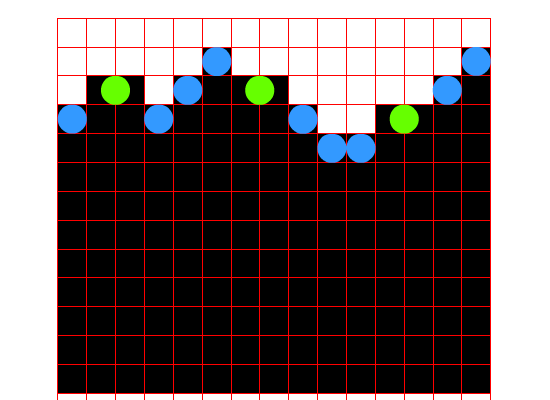
\includegraphics[width=0.6\textwidth]{TooFewSamples02}
	\caption{Beispiel: Mehr Pixel als Sample}
	\label{fig:gauge}
\end{figure}

Für den Fall mehr Sample als Pixel, wird wiederum durch jeden Pixel iteriert und berechnet welche Sample für das momentane Pixel relevant sind. Dabei werden stets 2 Pixel gleichzeitig betrachtet, da für die Darstellung das lokale Minimum und Maximum gezeichnet wird.\\

\begin{figure}[ht]
	\centering
	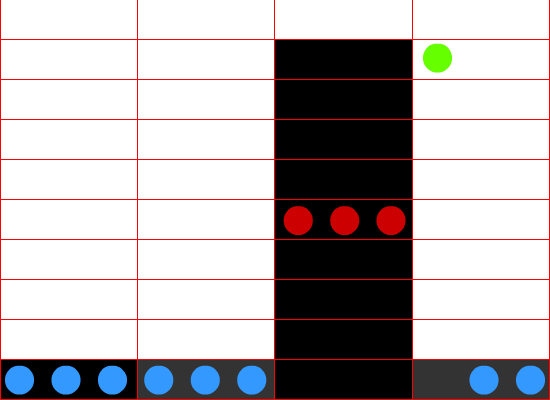
\includegraphics[width=0.6\textwidth]{TooManySamples030001}
	\caption{Beispiel: Mehr Pixel als Sample 01}
	\label{fig:gauge}
\end{figure}
In diese Abbildung zum Beispiel sind für die rechten zwei Pixel Spalten sechs Sample relevant. Drei rote Sample mit mittel hohen Wert, ein grünes Sample mit einem sehr hohen Wert und zwei blaue Sample mit niedrigen Werten.\\
Das Minimum und Maximum wird bestimmt. Das grüne Sample entspricht dem Maximum, während eins der blauen Sample das Mimimum entspricht. Da das Maximum (grün) rechts vom Minimum (blau) ist, wird entsprechend die linke Spalte das Maximum und die rechte Spalte das Minimum anzeigen.\\
\chapterauthor{Bernd Krupinski}
\subsection{Gauge Control Implementierung}

Die Implementierung der Gauge Control erfolgte in der Windows Presentation Foundation (WPF) über eine Custom Control. Zur Darstellung der Skala(1) und dem Zeiger(2) wurden jeweils ein Canvas verwendet. Ein Canvas stellt in WPF eine Zeichenoberfläche dar.\\



Das Control stellt eine Reihe an Variablen zur Verfügung. Diese ermöglichen es dem Entwickler das Control mit Hilfe von wenigen Zeilen Code stark anzupassen. 
\begin{figure}[ht]
	\centering
	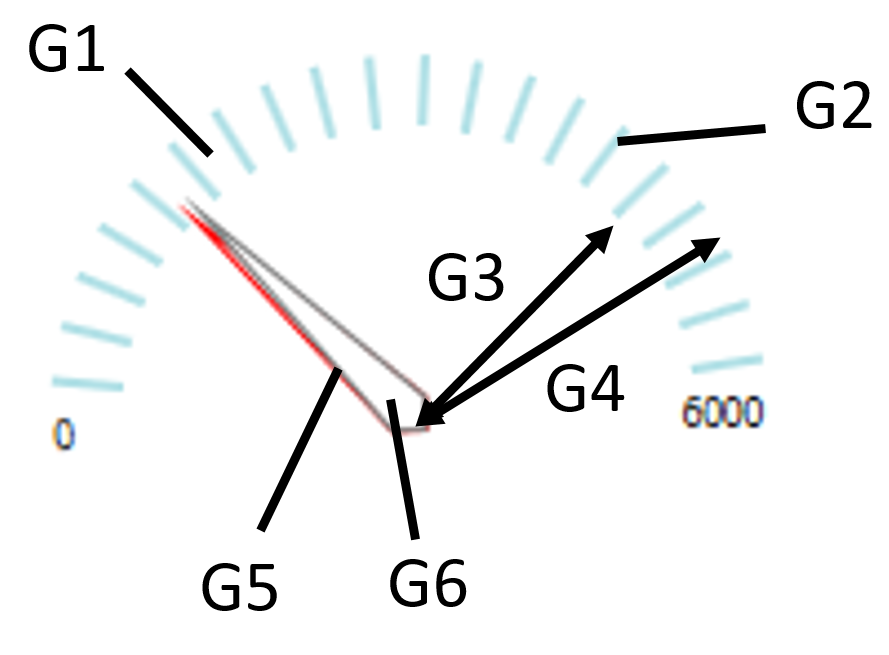
\includegraphics[width=0.6\textwidth]{GaugeDetails}
	\caption{Gauge Control Details}
	\label{fig:gauge}
\end{figure}
Umfassen dabei sind visuelle Parameter wie Kreishintergrundfarbe(G1), Strichlänge, Strichfarbe, Strichanzahl(G2), innerer Radius(G3), Nadellänge, Nadelfarbe(G6) oder Nadelfüllfarbe(G5). Zusätzlich dazu funktionelle Parameter wie Maximalwert, Minimalwert, aktueller Wert etc.\\\\

Das Canvas Control benutzt den Render Zyklus von WPF. Das heißt dass von unserer Seite das Canvas nur geändert werden muss, sollte einer der genannten Variablen sich verändern, also ein neu zeichnen des Tachometers notwendig ist.\\
Dies geschieht in 2 Schritten. \\
\begin{itemize}
	\item Zeichnen des Hintergrunds (Canvas 1)
	\item Zeichnen der Nadel (Canvas 2)
\end{itemize}

Der Hintergrund besteht wiederum aus 2 Teilen. \\

\begin{itemize}
	\item Der kreisförmige Hintergrund.
	\item Halbkreis aus Strichen.
\end{itemize}
Während die Striche mit einer Menge an Strich-Formen entlang des inneren Radius mit der Länge Äußerer Radius(G4) - Innerer Radius, einfach gelöst wird, stellt der Hintergrund eine etwas interessante Problematik.\\
Zwar gibt es eine Ellipsen Form für WPF's Canvas Control, allerdings besteht die Anforderung aus keiner rein einfarbigen Ellipse, sondern stattdessen aus einer zwei geteilte Form wie unten abgebildet.
\begin{figure}[ht]
	\centering
	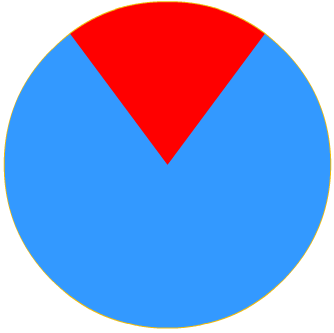
\includegraphics[width=0.6\textwidth]{GaugeForm}
	\caption{Gauge Control Details}
	\label{fig:gauge}
\end{figure}
Stattdessen wird ein Polygon benutzt. Ein Polygon ist eine mit einer Linie verbundene, Menge an Punkten. Optional kann die daraus entstehende Fläche mit einer Farbe gefüllt werden.\\
Um die gewünschte Form zu erzielen, werden 2 Polygone gezeichnet. Das eine (blau) umschließt das andere (rot) und bilden zusammen einen vollen Kreis.\\
\\
Die Nadel wird genau wie der Hintergrund über ein Polygon gezeichnet. Dabei wird die Nadel selbst auf dem Canvas stets richtung Osten gezeichnet. Damit die Nadel schließlich auf den entsprechenden Winkel zeigt, der den aktuellen Wert entspricht, wird nicht die Nadel schräg gezeichnet, sondern stattdessen das Canvas selbst über eine Rotations-Transformation gedreht.

